\documentclass[tikz,border=9pt]{standalone}
\usepackage{amsmath,amssymb}
\usetikzlibrary{arrows.meta,positioning,calc}
\begin{document}
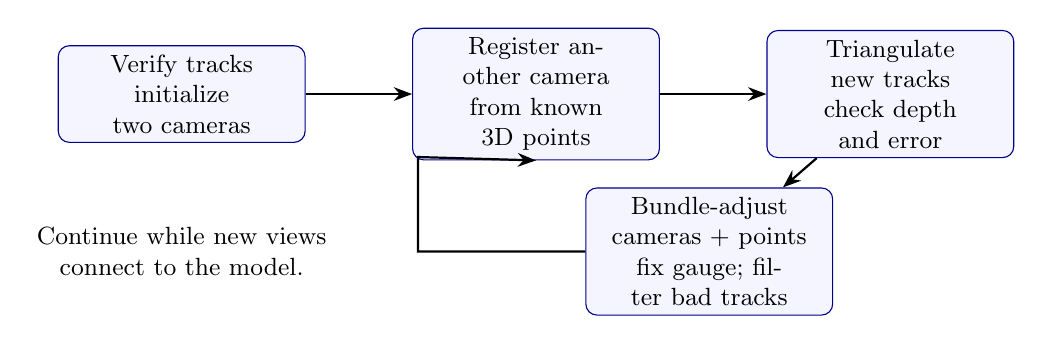
\begin{tikzpicture}[font=\small,arr/.style={-{Stealth},thick},box/.style={draw=blue!55!black,rounded corners,fill=blue!4,align=center,text width=2.9cm,minimum height=1.05cm}]

\node[box] (pair) at (0,0) {Verify tracks\\initialize two cameras};
\node[box] (pose) at (4.5,0) {Register another camera\\from known 3D points};
\node[box] (points) at (9,0) {Triangulate new tracks\\check depth and error};
\node[box] (ba) at (6.7,-2) {Bundle-adjust cameras + points\\fix gauge; filter bad tracks};
\draw[arr] (pair)--(pose);\draw[arr] (pose)--(points);\draw[arr] (points)--(ba);
\draw[arr] (ba.west)--(3,-2)--(3,-.8)--(pose.south);
\node[align=center] at (0,-2) {Continue while new views\\connect to the model.};

\end{tikzpicture}
\end{document}
